\section{Chapter 4 DeepNeuralNetwork}


\begin{frame}[fragile]{ここで話すこと}
\begin{itemize}
\item  ニューラルネットワークのイメージ \\
\item ニューラルネットワークの定義 \\
\item ニューラルネットワークの表現能力 \\
\item ニューラルネットワークの学習 \\
\item DeepLearningのチューニング
\end{itemize}
\end{frame}

\section{AND/ORでみるニューラルネットワーク}

\begin{frame}{ニューラルネットワークの絵}
\begin{center}
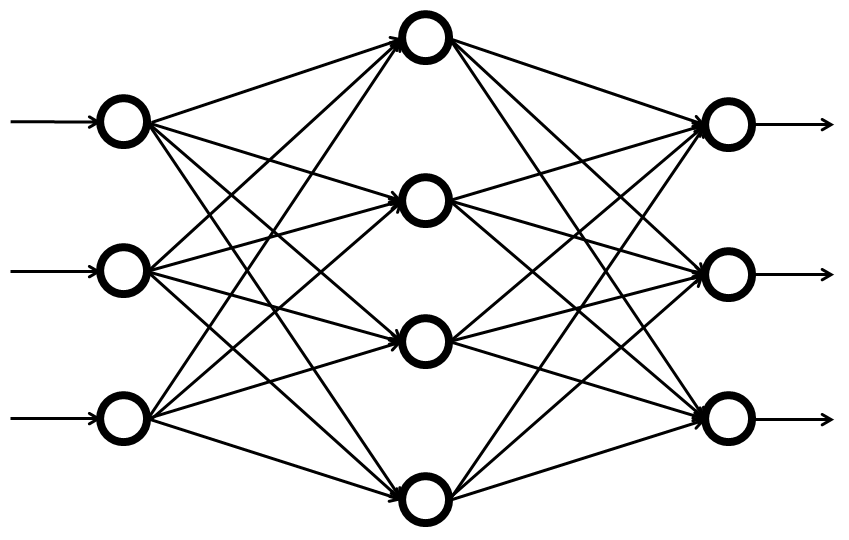
\includegraphics[width=8cm]{pic/dnn_sample.png}
\end{center}

\footnote{\url{http://nkdkccmbr.hateblo.jp/entry/2016/10/06/222245}より}
\end{frame}

\begin{frame}[fragile]{ニューラルネットワークの雰囲気}
  \begin{itemize}
    \item $\bullet$: ユニット
    \item $\bullet$の列: 層
    \item 層を重ねて予測をする.
  \end{itemize}
\end{frame}

\begin{frame}[fragile]{二層のパーセプトロンの定義}

\begin{screen}
\begin{dfn}
以下を満たすものを二層のパーセプトロンといいます.
\begin{itemize}
\item 入力: $x_1, x_2$
\item パラメータ: $w_1, w_2, \theta$
\item 出力:
\begin{equation*}
y = \left\{
\begin{array}{ll}
0 & w_1 x_1 + w_2 x_2 < \theta \\
1 & w_1 x_2 + w_2x_2 \ge \theta
\end{array}
\right.
\end{equation*}
\end{itemize}
\end{dfn}
\end{screen}
\end{frame}


\begin{frame}[fragile]{二層のパーセプトロンの性質}
\begin{itemize}
\item 実現できるもの
  \begin{itemize}
  \item AND
  \item OR
  \item NAND
  \end{itemize}
\item 実現できないもの
   XOR
\end{itemize}

\textbf{注意}: 入力は0,1のみを考える
\end{frame}

\begin{frame}[fragile]{AND}

実現例
\begin{itemize}
  \item $w_1 = w_2 = 0.5$
  \item $\theta = 0.7$
\end{itemize}

実際計算してみる
\begin{itemize}
\item $(x_1, x_2)$が(0,0),(1,0),(0,1)のときは高々0.5
\item (1,1)のときは1となります.
\item $\theta$の条件を考えると確かに`AND`.
\end{itemize}

\end{frame}

\begin{frame}[fragile]{OR}

実現例
\begin{itemize}
  \item $w_1 = w_2 = 0.5$
  \item $\theta = 0.3$
\end{itemize}
実際計算してみると

\begin{itemize}
\item $(x_1, x_2)$が(1,1),(1,0),(0,1)のときは少なくとも0.5
\item (0,0)のときは0となります.
\item $\theta$の条件を考えると確かに`OR`.
\end{itemize}
\end{frame}


\begin{frame}[fragile]{NAND}
NANDはANDを反転させたもの. \\
実現例
\begin{itemize}
  \item $w_1 = w_2 = -0.5$
  \item $\theta = - 0.7$
\end{itemize}
\end{frame}


\begin{frame}[fragile]{二層のパーセプトロンの気持ち}
\begin{itemize}
\item 二層のパーセプトロンは超平面で分離する = 線形モデル.
\item AND/NAND/OR等のモデルはかける
\item XORのような非線形なものはかけない
\end{itemize}
\end{frame}

\begin{frame}[fragile]{XOR}
XOR: $ \{0, 1\} \times  \{0, 1\} \to  \{0, 1\}$
\begin{itemize}
  \item $(0, 1), (1, 0)$の時1
  \item $(1, 1),(0, 0)$の時0
\end{itemize}

XOR二層のパーセプトロンでは表せない \\
もし表せたとすると,矛盾することを示します.
\end{frame}


\begin{frame}[fragile]{XORが表せない証明}
$(1, 0),(0, 1)$で$w_1x_1 + w_2x_2 \ge \theta$
\begin{itemize}
    \item $(1, 0)$の時$w_1 \ge \theta$
    \item $(0, 1)$の時$w_2 \ge \theta$
\end{itemize}
$(0, 0),(1, 1)$で$w_1x_1 + w_2x_2 < \theta$
\begin{itemize}
\item $(0, 0)$の時,$0 < \theta$
\item $(1, 1)$の時,$w_1 + w_2 < \theta$
\end{itemize}

この時、$w_1 \ge \theta$,$w_2 \ge \theta$より
\begin{itemize}
\item $w_1 + w_2 \ge 2\theta$となり,$0 < \theta$より
\item $w_1 + w_2 \ge 2 \theta  > \theta$となり
\end{itemize}
$(1,1)$の場合に条件と矛盾する.
\end{frame}


\begin{frame}[fragile]{三層での表現方法}
ただし、これを三層のパーセプトロンにすれば実現できます.

\begin{equation*}
\begin{array}{ll}
s_1 =  NAND(x_1, x_2) \\
s_2 =  OR(x_1, x_2) \\
XOR(x_1, x_2) = AND(s_1, s_2)
\end{array}
\end{equation*}
\end{frame}


\begin{frame}[fragile]{XORの結果の確認}
\begin{itemize}
\item (1,1)のとき
  \begin{itemize}
  \item $s_1 = NAND(1,1) = 0, s_2 = OR(1, 1) = 1$
  \item $AND(s_1, s_2) = AND(0, 1) = 0$
  \end{itemize}
\item (1,0)のとき
  \begin{itemize}
  \item $s_1 = NAND(1,0) = 1, s_2 = OR(1, 0) = 1$
  \item $AND(s_1, s_2) = AND(1, 1) = 1$
  \end{itemize}
\item (0,1)のとき
  \begin{itemize}
  \item $s_1 = NAND(0,1) = 1, s_2 = OR(0, 1) = 1$
  \item $AND(s_1, s_2) = AND(1, 1) = 1$
  \end{itemize}
\item (0,0)のとき
  \begin{itemize}
  \item $s_1 = NAND(0,0) = 1, s_2 = OR(0, 0) = 0$
  \item $AND(s_1, s_2) = AND(1, 0) = 0$
  \end{itemize}
\end{itemize}
\end{frame}


\begin{frame}[fragile]{まとめ}
\begin{itemize}
\item AND/OR/NAND等は二層のパーセプトロンで書ける
\item XORは二層のパーセプトロンでかけない.
\item XORは三層はパーセプトロンでかくことができる
\item 三層パーセプトロンは二層パーセプトロンを必ず表せる.
\end{itemize}
\end{frame}


\begin{frame}[fragile]{演習}
XORをpythonで実装し,正解を確認してください.
\end{frame}


\section{ニューラルネットワークの定義}


\begin{frame}[fragile]{すすめ方}
ニューラルネットワークを二層、三層、多層で形式的に定義する.

\end{frame}


\begin{frame}[fragile]{二層のニューラルネットワークの定義}
行列$W_1 \in M_{n_0 n_1}(\mathbb{R})$とベクトル$b_1  \in \mathbb{R}^{n_1}$と$\sigma:\mathbb{R}^{n_1}  \to \mathbb{R}^{n_1}$が存在し,

\begin{equation*}
F = \sigma \circ f_{W_1,b_1}
\end{equation*}

と書ける時,関数$F:\mathbb{R}^{n_0} \to \mathbb{R}^{n_1}$を \textbf{二層のニューラルネットワーク}という.
ただし,$f_{W_1,b_1}:\mathbb{R}^{n_{0}} \to \mathbb{R}^{n_1}$は$ x \mapsto W_ix+b_i$で定める写像である.
\end{frame}


\begin{frame}[fragile]{Softmax回帰は二層のニューラルネットワーク}
$x \in \mathbb{R}^2, w \in \mathbb{R}^{2 \times 2}$とする.$f:  \mathbb{R}^2 \to  \mathbb{R}^2$に対して,

\begin{equation*}
  f(x) = \mathrm{softmax}(w \cdot x)
\end{equation*}

\textbf{注意}: 分類の場合はさらに$\mathrm{argmax}$で値域を変えて場合もある.
\end{frame}


\begin{frame}[fragile]{三層のニューラルネットワークの定義}
行列$W_1 \in (\mathbb{R}^{n_0 \times n_1}),W_2 \in (\mathbb{R}^{n_1 \times n_2})$とベクトル$b_1  \in \mathbb{R}^{n_1} ,b_2 \in \mathbb{R}^{n_2}$と$ \sigma:\mathbb{R}^{n_2}  \to \mathbb{R}^{n_2}$が存在し,
\begin{equation*}
F = \tau \circ f_{W_2,b_2} \circ \sigma \circ f_{W_1,b_1}
\end{equation*}

と書ける時,関数$F:\mathbb{R}^{n_0} \to \mathbb{R}^{n_2}$を \textbf{三層のニューラルネットワーク}という.
ただし,$f_{W_i,b_i}:\mathbb{R}^{n_{i-1}} \to \mathbb{R}^{n_i}$は$ x \mapsto W_ix+b_i$で定める写像である.
\end{frame}


\begin{frame}[fragile]{ニューラルネットワークの絵(再掲)}
![](https://cdn-ak.f.st-hatena.com/images/fotolife/n/nkdkccmbr/20161006/20161006215155.png)
この画像は[人工知能であそぶ](http://nkdkccmbr.hateblo.jp/entry/2016/10/06/222245)で公開されていたものを使わせていただきました.

\end{frame}


\begin{frame}[fragile]{ニューラルネットワークのグラフ構造}
\begin{itemize}
\item グラフは点と線の組
\item $\mathbb{R}^n \to \mathbb{R}^{m}$の場合,n個の点とm個の点を結ぶ
\item ニューラルネットワークの絵はグラフ
  \begin{itemize}
  \item 単純グラフ(ループ、多重辺のない)
  \item 重み付き(重みが行列の掛け算に相当)
  \item 活性化関数を加えることも
  \end{itemize}
\end{itemize}

\end{frame}


\begin{frame}[fragile]{$L$層ニューラルネットワーク}
\begin{itemize}
  \item 2層3層のニューラルネットワークから層を増減させることで$L$層ニューラルネットワークを定義できる.
  \item 入力層と出力層が必要なので最低でも2層は必要.
  \item グラフとしては行列の重みしかないが、実際には2層,3層と同様に活性化関数がある.
\end{itemize}
\end{frame}


\begin{frame}[fragile]{隠れ層の活性化関数}
以下が有名
\begin{itemize}
\item sigmoid :$\sigma(x) = \frac{1}{1 + e^{-x}}$
\item: $ReLU(x) = \max\{x, 0\}$
\end{itemize}

だが、sigmoidは勾配消失問題があるため、ReLUが実質一強状態.
ReLUの亜種はいくつかある。
\end{frame}


\begin{frame}[fragile]{演習}
以下を微分せよ.ただし、$ReLU$は$x=0$では劣微分を求めてください.
\begin{itemize}
\item  sigmoid :$\sigma(x) = \frac{1}{1 + e^{-x}}$
\item ReLU: $ReLU(x) = \max\{x, 0\}$
\end{itemize}
\end{frame}


\section{深層学習の表現能力}

\begin{frame}[fragile]{機械学習モデルの表現能力とは}
\begin{itemize}
\item どれだけ難しい問題だとしても学習できるか
\item つまり,うまいパラメータをとったときにどの精度になるか
  \begin{itemize}
  \item 分類:空間を分割できる数がどれだけ多いか?
  \item 回帰:真の関数との誤差≒損失をどこまで小さくできるか?
  \end{itemize}
\end{itemize}
\end{frame}


\begin{frame}[fragile]{万能近似定理}
一言でいうと,ニューラルネットワークは全ての連続関数を近似できる.
厳密に言うと,
\begin{theorem}
定義域がコンパクトな連続関数全体の空間上,$\sigma,\tau$にシグモイド関数を取った三層のニューラルネットワーク全体のなす集合はsupノルムが定める位相に対して稠密である.
\end{theorem}
\end{frame}


\begin{frame}[fragile]{万能近似定理の用語}
\begin{itemize}
\item supノルムが定める位相: 関数の間の距離を定める方法の一つ.
  関数同士の近さを図る場合に成分ごとの絶対値$|f(x)_i-g(x)_i|$の最大値で定めたもの.
\item 稠密: 全てとは限らないが、いくらでも近いものがある.
  例) 有理数は実数の中で稠密.
\item コンパクト: 有界な閉集合のこと.例えば $[0, 1]$
\end{itemize}
\end{frame}


\begin{frame}[fragile]{深層の強み1}
Montufar, Pascanu, Cho, Bengio(2014年)
\begin{theorem}
隠れ層の活性化関数がReLUのニューラルネットワークを考える.
\begin{itemize}
  \item 隠れ層の数を$L$
  \item 隠れ層のユニットの数を$n$
  \item 入力の次元を$d$
\end{itemize}
このとき,入力空間は最大で$\displaystyle\left(\frac{n}{d}\right)^{L-1}\sum_{i=0}^{d}\binom{n}{i}$個の領域に分割可能
\end{theorem}

\begin{itemize}
\item つまり、これだけ分類できる可能性がある.
\item 層の数に指数的に伸びる
\item ユニットの数に対しては多項式的な伸びる
\end{itemize}
\end{frame}


\begin{frame}[fragile]{深層の強み2}
\begin{theorem}[Imaizumi, Fukumizu(2018年]
十分なユニット数と十分な深さをもつ深層ニューラルネットワークは、不連続な関数、特に区分的に滑らかな関数を表現できる。
\end{theorem}

区分的に滑らかな関数はRBFカーネルのサポートベクトルマシンでは表現できず,真に強い、
\end{frame}


\section{ニューラルネットワークの学習方法}


\begin{frame}[fragile]{学習の基本的な考え方}
\begin{itemize}
\item 損失が最小になるようにパラメータを調整する
\item 深層学習の学習の特徴
  \begin{itemize}
  \item パラーメータが多い
  \item データが多い(少ないと学習できないことも多い)
  \item データもパラメータも多いので、勾配降下の計算が大変
    \begin{itemize}
    \item 空間(メモリ的にも)
    \item 時間(計算時間的にも)
    \end{itemize}
  \end{itemize}
\item 方針
  \begin{itemize}
  \item 学習のアルゴリズムを工夫する(誤差逆伝播法)
  \item 学習データを工夫する(確率的勾配降下)
  \end{itemize}
\end{itemize}
\end{frame}

\section{学習のアルゴリズムを工夫する(誤差逆伝播法)}

\begin{frame}[fragile]{誤差逆伝播法}
\begin{itemize}
\item 勾配降下では損失関数のパラメータでの偏微分を行う
\item ニューラルネットワークでは偏微分すると後ろの層の偏微分が出てくる.
\item 後ろから計算させて計算量を減らすことを誤差逆伝播法という
\end{itemize}
\end{frame}


\begin{frame}[fragile]{誤差逆伝搬の計算方法}
$\ell = (y - \sigma \circ W^c \circ \sigma \circ W^{b} \circ \sigma \circ W^{a}(x))^2$の場合を考える
\begin{itemize}
  \item パラメータは$W^c, W^b, W^a$
  \item $f^c(x) = (\sigma \circ W^cx)$
  \item $f^b(x) = (\sigma \circ W^bx)$
  \item $f^a(x) = (\sigma \circ W^ax)$
  \item $u_a = W^ax, z_a = f^a(x)$
  \item $u_b = W^bz_a, z_b = f^b(z_a)$
  \item $u_c = W^cz_b, z_c = f^c(z_b)$
  \item $\ell = (y - f_c(z_b))^2 = (y - f_c(f_b(z_a))^2 = (y - f_c(f_b(f_a(x))))^2$
\end{itemize}
\end{frame}


\begin{frame}[fragile]{偏微分の計算}
\begin{align*}
\frac{\partial \ell}{\partial W^c_{11}} & =  \frac{\partial \ell}{\partial z_c}\cdot \frac{\partial f_c}{\partial W^c_{11}}= 2(y - z_c) \cdot \frac{\partial f_c}{\partial W^c_{11}} \\
  & = 2(y- z_c) \cdot \frac{\partial \sigma}{\partial u_c} \frac{\partial u_c}{\partial W^c_{11}} = 2(y-z_c)(\sigma(u_c)(1 - \sigma(u_c))(x_1)
\end{align*}
\begin{equation*}
\frac{\partial \ell}{\partial W^b_{11}} =  \frac{\partial \ell}{\partial z_c}\cdot  \frac{\partial f_c}{\partial z_b}\frac{\partial f_b}{\partial W^b_{11}}
\end{equation*}
\begin{itemize}
  \item 右辺の初項は上の偏微分計算の中で求めている.
  \item 毎回ラスト2項だけ新しく計算して求めていく.
\end{itemize}

\begin{itemize}
\item Jacobi行列の積になっていることには注意
\end{itemize}
\end{frame}


\begin{frame}[fragile]{演習}
実際に3層のNNに対して,誤差逆伝搬を使い,損失の微分を計算しよう.
\begin{itemize}
\item 活性化関数は全て$sigmoid$
\item 入力(1,1), 出力(1,0)
\item 損失は二乗誤差
\end{itemize}
\begin{equation*}
W_1 = \begin{pmatrix}
2 & 3 \\
1 & 4 
\end{pmatrix}
\end{equation*}

\begin{equation*}
W_2 = \begin{pmatrix}
3 & -1 \\
0 & 4 
\end{pmatrix}
\end{equation*}
\end{frame}

\section{学習データを工夫する(確率的勾配降下)}
\begin{frame}[fragile]{確率的勾配降下}
\begin{itemize}
\item データを小さいサイズに分割して、勾配降下させる.
\item 全てのデータは使わない.
\item 厳密には
  \begin{itemize}
  \item 確率的勾配降下はサイズが一つ
  \item バッチ型勾配降下はサイズが1以上をさす
  \end{itemize}
\item PytorchなどのクラスはバッチでもSGDになる.
  (バッチ型に対してSGDということも多い.)
\end{itemize}
\end{frame}


\begin{frame}[fragile]{普通の勾配降下法(復習)}
\begin{itemize}
\item 例えばデータが1000個あるとする
\item 普通の損失は$L(w;D)  = \sum_{i = 1}^{1000} \ell(w, x_i, y_i)$
\item これの勾配を計算する.
\item データが多すぎるとメモリや計算時間で限界が来る.
\end{itemize}
\end{frame}


\begin{frame}[fragile]{確率勾配降下法}
例えばデータが1000個あるとする。確率的勾配降下はこれをデータを10個の組にランダムに分割する. \\
$j=1$から10まで分割する場合
\begin{equation*}
  L_j(w;D)  = \sum_{i = 100j +1}^{100j + 100} \ell(w, x_i, y_i)
\end{equation*}
\begin{itemize}
\item  メリット: 一度の計算が小さくなる.
\item 注意: データが毎回変わるため、パラメータが同じでも損失の値が変わる.
\end{itemize}
\end{frame}


\begin{frame}[fragile]{確率的勾配降下の理論保証}
  TBD
\end{frame}

\begin{frame}[fragile]{確率的勾配降下法の亜種}
方式例
\begin{itemize}
  \item RMSProp
  \item Adagrad
  \item ADAM
\end{itemize}
現状
\begin{itemize}
  \item ADAMがいいSGDがいい等が度々議論(論文)になる
  \item 画一的な結論は出ていない.
\end{itemize}
\end{frame}

\section{ニューラルネットワークのチューニング}

\begin{frame}{勾配消失問題}
Sigmoidのは微分は真に1未満になる.
そのためSigmoidを活性化関数とすると微分が非常に小さい値になることもある.
\begin{itemize}
  \item  $\sigma(x)$の微分は$\sigma(x)(1 - \sigma(x))$
  \item $\sigma(x) < 1$よりどんどん小さくなる.
\end{itemize}
これを勾配消失問題という. 

$\Rightarrow$ 対策:ReLUのような関数を使う.
\end{frame}


\begin{frame}[fragile]{チューニングの方法}
Overfitting
\begin{itemize}
  \item 重み減衰
  \item Dropout
  \item ノイズ混入
  \item Early Stopping
\end{itemize}
勾配消失問題
\begin{itemize}
  \item BatchNormalization
\end{itemize}
\end{frame}


\begin{frame}[fragile]{重み減衰}
以下のようにパラメータを更新すること
\begin{equation*}
  w_{t+1} =  w_{t} - \eta \frac{\partial \ell}{\partial w}(w_t) - \eta \lambda w_t
\end{equation*}
$L^2$正則化に相当する.
つまり,ロスを$\ell$ではなく$\ell + \lambda ||w||^2$にしたもの.

\begin{minted}[frame=lines, fontsize=\footnotesize, breaklines=true, bgcolor=black]{python}
optimizer = torch.optim.SGD(model.parameters(), lr=0.1, momentum=0.9, weight_decay=0.01)
optimizer.zero_grad()
loss_fn(model(input), target).backward()
optimizer.step()
\end{minted}
\end{frame}


\begin{frame}[fragile]{Dropout}
- ランダムに入力を0に変更する.

\begin{minted}[frame=lines, fontsize=\footnotesize, breaklines=true, bgcolor=black]{python}
m = nn.Dropout(p=0.2)
input = torch.randn(20, 16)
output = m(input)
print(output)
\end{minted}

\end{frame}


\begin{frame}[fragile]{Batch Normalization}
- バッチ内で入力を平均0,分散1のminibatchに変換する.
\begin{minted}[frame=lines, fontsize=\footnotesize, breaklines=true, bgcolor=black]{python}
# With Learnable Parameters
m = nn.BatchNorm1d(100)
# Without Learnable Parameters
m = nn.BatchNorm1d(100, affine=False)
input = torch.randn(20, 100)
output = m(input)
\end{minted}
- 推論時は学習時の変換に合わせる.

\end{frame}
\begin{frame}[fragile]{Early Stopping}
- 誤差が十分に小さい場合に学習をやめる.
\begin{minted}[frame=lines, fontsize=\footnotesize, breaklines=true, bgcolor=black]{python}
from torchsample.callbacks import EarlyStopping

callbacks = [EarlyStopping(monitor='val_loss', patience=5)]
model.set_callbacks(callbacks)
\end{minted}
\end{frame}
\begin{frame}[fragile]{ノイズ混入}
\begin{itemize}
\item 敢えて誤ったデータを入れると適切に正則化する場合がある.
\item 正直いって悲しいが割とある...
\end{itemize}
\end{frame}


\begin{frame}[fragile]{演習}
- PytorchでDNNを使いMNISTの分類を行ってください.

\end{frame}
\begin{frame}[fragile]{今後作りたいなと思っているもの}
\begin{itemize}
\item CNN(AlexNet): CNNの基本
\item ReSNet: CNNの重要なもの
\item M2Det: 物体検出で大事そうなので.
\item GAN: 生成モデル一個ぐらいは
\item DeepFM: レコメンドの一つ
\item Collaborative Metric Learning: レコメンドの一つ
\item Are We Really Making Much Progress? A Worrying Analysis of Recent Neural Recommendation Approaches (RecSys 2019): RecSys 2019のトップ論文
\end{itemize}
\end{frame}

\section{ChainerのPythonコードを追う}

\begin{frame}[fragile]{DeepLearningの処理をおう}
対象
\begin{itemize}
\item  Linear: (行列をかける)
\item SGD: (勾配降下)
\end{itemize}

Chainerにした理由
\begin{itemize}
\item 雰囲気でも追える
\item 他はPython部分に処理が少ない.
\end{itemize}
\end{frame}


\begin{frame}[fragile]{Linear}
\url{https://github.com/chainer/chainer/blob/eb8dee82942ef3c1b9ef6f89d7fe93ed8e6bb819/chainer/functions/connection/linear.py#L13}

\begin{minted}[frame=lines, fontsize=\footnotesize, breaklines=true, bgcolor=black]{python}
class LinearFunction(function_node.FunctionNode):
    #intel cpuでの高速化
    _config_use_ideep = None
    _supports_static_optimizations = True
\end{minted}
以降は関係ない部分は省略する.
\end{frame}


\begin{frame}[fragile]{forward}
\begin{minted}[frame=lines, fontsize=\footnotesize, breaklines=true, bgcolor=black]{python}
def forward(self, inputs):
    if len(inputs) == 3:
        x, W, b = inputs
    else:
        (x, W), b = inputs, None
    xp = backend.get_array_module(x)
    y = xp.empty((x.shape[0], W.shape[0]), dtype=x.dtype)
    # 行列をかける
    self.static_linear_no_bias(xp, x.dtype == W.dtype, inputs=[x, W], outputs=[y])
    if len(inputs) == 3:
        self.static_add_bias(inputs=[b], outputs=[y])
    
    self.retain_inputs((0, 1))  # b is not retained
    return y,
\end{minted}
\end{frame}
        

\begin{frame}[fragile]{static\_linear\_no\_bias}
\begin{minted}[frame=lines, fontsize=\footnotesize, breaklines=true, bgcolor=black]{python}
@static_code
def static_linear_no_bias(self, xp, optimized, inputs, outputs):
    x, W = inputs
    y = outputs[0]

    if optimized:
        # Note: We can only call this function when both x and W
        # have the same dtype. Otherwise, the output type (for y)
        # may not be as expected (i.e., not the same dtype as x).
        xp.dot(x, W.T, out=y)
    else:
        y[:] = x.dot(W.T).astype(x.dtype, copy=False)
\end{minted}
\end{frame}


\begin{frame}[fragile]{結局やっていること}
\begin{itemize}
\item ただ$x, W$の行列をかけている
\item $x$がバッチになっても対応している.
\item バイアスあり、なしともに対応している.
\item 高速化の工夫をしている.
\end{itemize}


\end{frame}
\begin{frame}[fragile]{backward}
\begin{minted}[frame=lines, fontsize=\footnotesize, breaklines=true, bgcolor=black]{python}
def backward(self, indexes, grad_outputs):
    x, W = self.get_retained_inputs()
    gy, = grad_outputs
    ret = []
    
    if 0 in indexes:
        gx, = LinearGradData().apply((W, gy))
        ret.append(chainer.functions.cast(gx, x.dtype))
    if 1 in indexes:
        gW, = LinearGradWeight(W.dtype).apply((x, gy))
        ret.append(chainer.functions.cast(gW, W.dtype))
    if 2 in indexes:
        gb = chainer.functions.sum(gy, axis=0)
        ret.append(gb)

    return ret
\end{minted}

\end{frame}


\begin{frame}[fragile]{get\_retaind\_inputs()}
\begin{minted}[frame=lines, fontsize=\footnotesize, breaklines=true, bgcolor=black]{python}
    def get_retained_inputs(self):
        retained_inputs = []
        for index in self._input_indexes_to_retain:
            input = self.inputs[index]
            if input.data is None:
                retained_inputs.append(None)
            else:
               retained_inputs.append(input.get_variable())
        return tuple(retained_inputs)
\end{minted}
\end{frame}


\begin{frame}[fragile]{SGD}
\begin{minted}[frame=lines, fontsize=\footnotesize, breaklines=true, bgcolor=black]{python}
class SGD(optimizer.GradientMethod):
    """Vanilla Stochastic Gradient Descent.
    Args:
        lr (float): Learning rate.
    """

    def __init__(self, lr=_default_hyperparam.lr):
        super(SGD, self).__init__()
        self.hyperparam.lr = lr

    lr = optimizer.HyperparameterProxy('lr')

    def create_update_rule(self):
        return SGDRule(self.hyperparam)
\end{minted}
\end{frame}


\begin{frame}[fragile]{SGDRule 初期化}
\begin{minted}[frame=lines, fontsize=\footnotesize, breaklines=true, bgcolor=black]{python}
class SGDRule(optimizer.UpdateRule):

    """Update rule of vanilla stochastic gradient descent.
    """
    is_elementwise = True

    _kernel = None

    def __init__(self, parent_hyperparam=None, lr=None):
        super(SGDRule, self).__init__(
            parent_hyperparam or _default_hyperparam)
        if lr is not None:
            self.hyperparam.lr = lr
\end{minted}
\end{frame}


\begin{frame}[fragile]{SGDRule 更新}
パラメータの更新を行う.

\begin{minted}[frame=lines, fontsize=\footnotesize, breaklines=true, bgcolor=black]{python}
    def update_core_cpu(self, param):
        grad = param.grad
        if grad is None:
            return
        if isinstance(param.data, intel64.mdarray):
            param.data.inplace_axpby(1.0, -self.hyperparam.lr, grad)
        else:
            # パラメーターを更新した
            param.data -= self.hyperparam.lr * grad
\end{minted}
\end{frame}
